\begin{tikzpicture}
  \tkzTabInit{ / 1} { , }
\end{tikzpicture}
---
\begin{tikzpicture}
  \tkzTabInit[lgt=3]{ $x$ / 1} { $1$ , $3$ }
\end{tikzpicture}
---
\begin{tikzpicture}
  \tkzTabInit[lw=2pt]{ / 1} { , }
\end{tikzpicture}
---
\begin{tikzpicture}
  \tkzTabInit[nocadre]{ / 1, /1, /1} { , }
\end{tikzpicture}
---
\begin{tikzpicture}
  \tkzTabInit{$x$ / 1 , $f(x)$ / 1}{$0$, $6$, $+\infty$}
\end{tikzpicture}
---
\begin{tikzpicture}
  \tkzTabInit[color, colorT = yellow!20, colorC = red!20, colorL = green!20, colorV = lightgray!20, lgt = 1, espcl = 2.5] {$t$/1,$a$/1,$b$/1,$c$/1,$d$/1} {$\alpha$,$\beta$,$\gamma$}
\end{tikzpicture}
---
\begin{tikzpicture}
  \tkzTabInit[lgt=6,espcl=7]
  {$x$/0.75,
  $x-1.5$/0.75}
  {$-\infty$,$+\infty$}
\end{tikzpicture}
---
\begin{tikzpicture}
  \tkzTabInit[espcl=1.5] {$x$ / 1 ,$f(x)$ /1 } {$v_1$ , $v_2$ , $v_3$ }
  \tkzTabLine{ , , , , }
\end{tikzpicture}
---
\begin{tikzpicture}
  \tkzTabInit[espcl=1.5] {$x$ / 1 ,$f(x)$ /1 } {$v_1$ , $v_2$ , $v_3$ }
  \tkzTabLine{ t, , t , ,t }
\end{tikzpicture}
---
\begin{tikzpicture}
  \tkzTabInit[espcl=1.5] {$x$ / 1 ,$f(x)$ /1 } {$v_1$ , $v_2$ , $v_3$ }
  \tkzTabLine{ z, , z , ,z }
\end{tikzpicture}
---
\begin{tikzpicture}
  \tkzTabInit {$x$ /1, $f(x)$ /1, $g(x)$ /1} {$0$,$E$,$+\infty$}
\end{tikzpicture}
---
\begin{tikzpicture}
  \tkzTabInit {$x$ / 1 ,$f(x)$ /1}
  {$0$,$1$}
  \tkzTabLine{,$u(x)\\ v(x)$,}
\end{tikzpicture}
---
\begin{tikzpicture}
  \tkzTabInit{$x$ / 1 , $f(x)$ / 1}{$0$, $6$, $8$, $+\infty$}
  \tkzTabLine{z, -, d, h, d, +, }
\end{tikzpicture}
---
\begin{tikzpicture}
  \tkzTabInit{$x$ / 1 , $ax + b$ / 1}{$-\infty$, $-\dfrac{b}{a}$, $+\infty$}
  \tkzTabLine{, \text{signe de } a, z, \text{signe de } -a, }
\end{tikzpicture}
---
\begin{tikzpicture}
  \tkzTabInit{$x$ / 1 , $|x|$ / 1}{$-\infty$, $0$, $+\infty$}
  \tkzTabLine{, -x, z, x, }
\end{tikzpicture}
---
\begin{tikzpicture}
  \tkzTabInit[espcl=1.5] {$x$ / 1,$g(x)$ / 1} {$0$,$1$,$2$}
  \tkzTabLine{d,+,0,-,d}
\end{tikzpicture}
---
\begin{tikzpicture}
  \tkzTabInit[lgt=1.5,espcl=1.75] {$x$ / 1,$f'(x)$ / 1} {$-\infty$,$0$,$+\infty$}
  \tkzTabLine{,+,d,-}
\end{tikzpicture}
---
\begin{tikzpicture}
  \tkzTabInit[lgt=2,espcl=1.75] {$x$/1,$2-x$/1, $\vert 2-x \vert $/1} {$-\infty$,$2$,$+\infty$}
  \tkzTabLine{ , + , z , - , }
  \tkzTabLine{ , 2-x ,z, x-2, }
\end{tikzpicture}
---
\begin{tikzpicture}
  \tkzTabInit[color,espcl=1.5] {$x$ / 1,$g(x)$ / 1} {$0$,$1$,$2$,$3$}
  \tkzTabLine{z, + , d , h , d , - , t}
\end{tikzpicture}
---
\begin{tikzpicture}
  \tkzTabInit[lgt = 2.5, espcl = 3, deltacl = 0.7]{$x$ / 1 , $f(x)$ / 1}{$0$, $6$, $8$, $+\infty$}
  \tkzTabLine{z, -, d, h, d, +, }
\end{tikzpicture}
---
\begin{tikzpicture}
  \tkzTabInit[color, colorC = blue!15, colorL = green!15]
       {$x$ / 1 , $f(x)$ / 1}{$0$, $6$, $8$, $+\infty$}
  \tkzTabLine{z, -, d, h, d, +, }
\end{tikzpicture}
---
\begin{tikzpicture}
  \tkzTabInit[color, colorT = yellow!20, colorC = orange!20,
   colorL = green!20, colorV = lightgray!20] { /1 , /1}{ , }
\end{tikzpicture}
---
\begin{tikzpicture}
  \tkzTabInit[lgt=3,espcl=6]{$x$/1,$f'(x)$/1,$f(x)=\sqrt{x}$/2}{$0$,$+\infty$}
  \tkzTabLine{d,+,}
  \tkzTabVar{-/0,+/$+\infty$}
\end{tikzpicture}
---
\begin{tikzpicture}
  \tkzTabInit[lgt=3,espcl=6]{$x$/1,$f'(x)=-\dfrac{1}{\ x^2}$/1,$f(x)=\dfrac{1}{x}$/2}{$-\infty$,$0$,$+\infty$}
  \tkzTabLine{,-,d,-,}
  \tkzTabVar{+/0,-D+/$-\infty$/$+\infty$,-/0}
\end{tikzpicture}
---
\begin{tikzpicture}
  \tkzTabInit[espcl=6]{$x$/1,$\ln'(x)$/1,$\ln(x)$/2}{$0$,$+\infty$}
  \tkzTabLine{d,+,}
  \tkzTabVar{D-/$-\infty$,+/$+\infty$}
  \tkzTabVal{1}{2}{0.4}{1}{0}
  \tkzTabVal{1}{2}{0.67}{$E$}{1}
\end{tikzpicture}
---
\begin{tikzpicture}
  \tkzTabInit[espcl=6]{$x$ / 1,Signe de\\f'(x)/1, Variations de\\ $f$ / 3}
     {$0$ , $\pi$}
  \tkzTabLine{ , + , }
  \tkzTabVar{+/$1$ ,   -/$-1$ }
  \tkzTabVal{1}{2}{0.5}{$\frac{\pi}{2}$}{$0$}
\end{tikzpicture}
---
\begin{tikzpicture}
  \tkzTabInit{$x$ / 1 , $\cos(x)$ / 1, $\sin(x)$ / 1.5}{$0$, $\dfrac{\pi}{2}$, $\pi$}
  \tkzTabLine{, +, z, -, }
  \tkzTabVar{-/ 0, +/ 1, -/ 0}
\end{tikzpicture}
---
\begin{tikzpicture}
  \tkzTabInit{$x$ /1, $-\sin(x)$ /1, $\cos(x)$ /1.5} {$0$ , $\pi$}
  \tkzTabLine{, -,}
  \tkzTabVar{+/ 1, -/ -1}
  \tkzTabVal{1}{2}{0.5}{}{$0$}
\end{tikzpicture}
---
\begin{tikzpicture}
  \tkzTabInit{$x$ /1, $-\sin(x)$ /1, $\cos(x)$ /1.5} {$0$ , $\pi$}
  \tkzTabLine{, -,}
  \tkzTabVar{+/ 1, -/ -1}
  \tkzTabVal{1}{2}{0.5}{$\dfrac{\pi}{2}$}{0}
\end{tikzpicture}
---
\begin{tikzpicture}
  \tkzTabInit{$x$ / 0.8 , $g'(x)$ / 0.8, $g$ / 1.5}{$0$, $e$, $+\infty$}
  \tkzTabLine{, +, z, -, }
  \tkzTabVar{-/ -2, +/ $e-2$, -/ $-\infty$}
\end{tikzpicture}
---
\begin{tikzpicture}
  \tkzTabInit{$x$ / 1 , $f(x)$ / 2}{$-\infty$, $-5$, $-3$, $2$, $+\infty$}
  \tkzTabVar{-/ $-\infty$, +C/ $0$, +H/ $0$, D-/ $-10$, +/ $+\infty$}
\end{tikzpicture}
---
\begin{tikzpicture}
  \tkzTabInit{$x$ / 1 , $f(x)$ / 2}{$-\infty$, $-5$, $-3$, 0, $+\infty$}
  \tkzTabVar{-/ $-\infty$, +CD-/ $0$/ $2$, +D+/ $0$ /$0$, -V-/ $-2$ / $3$, +/ $+\infty$}
\end{tikzpicture}
---
\begin{tikzpicture}
  \tkzTabInit[]{$x$/1,$f'(x)$/1,$f(x)$/2}{$-\infty$,$-2$,$0$,2,$+\infty$}
  \tkzTabLine{,+,z,-,d,-,z,+,}
  \tkzTabVar{-/$-\infty$,+/-4,-D+/$-\infty$/$+\infty$,-/4,+/$+\infty$}
\end{tikzpicture}
---
\begin{tikzpicture}
  \tkzTabInit{$x$/1,$-\sin(x)$/1,$\cos(x)$/2}{$0$,$\pi$,$2\pi$}
  \tkzTabLine{z,-,z,+,z}
  \tkzTabVar{+/$1$,-/$-1$,+/$1$}
  \tkzTabVal{1}{2}{0.5}{$\dfrac{\pi}{2}$}{0}
  \tkzTabVal{2}{3}{0.5}{$\dfrac{3\pi}{2}$}{0}
\end{tikzpicture}
---
\begin{tikzpicture}
  \tkzTabInit{$x$ /1, $-\sin(x)$ /1, $\cos(x)$ /1.5} {$0$ , $\dfrac{\pi}{2}$, $\pi$}
  \tkzTabLine{, -, -1, -, }
  \tkzTabVar{+/ 1, R/, -/ -1}
  \tkzTabIma{1}{3}{2}{$0$}
\end{tikzpicture}
---
\begin{tikzpicture}
  \tkzTabInit[espcl=6]{$x$ / 1,Signe de\\f'(x)/1, Variations de\\ $f$ / 3}
     {$0$ ,$\frac{\pi}{2}$ , $\pi$}
  \tkzTabLine{ ,+,d,+, }
  \tkzTabVar{-/$0$ ,  +D-/$+\infty$/$-\infty$  , +/$0$ }
  \tkzTabVal{1}{2}{0.5}{$\frac{\pi}{4}$}{$1$}
  \tkzTabVal{2}{3}{0.5}{$\frac{3\pi}{4}$}{$1$}
\end{tikzpicture}
---
\begin{tikzpicture}
  \tkzTabInit[color,lgt=5,espcl=3] {$x$ / .8,$\Delta>0$ Le signe de $ax^2+bx+c$ /1.5} {$-\infty$,$x_1$,$x_2$,$+\infty$}
  \tkzTabLine{ , \genfrac{}{}{0pt}{0}{\text{signe de}}{a}, z , \genfrac{}{}{0pt}{0}{\text{signe}}{\text{opposé de}\ a}, z , \genfrac{}{}{0pt}{0}{\text{signe de}}{a}, }
\end{tikzpicture}
---
\begin{tikzpicture}
  \tkzTabInit[color,espcl=8] {$x$ /1, Signe de $\dfrac{1}{x}$ /1.5, Variation de $\ln$ /1.5} {$0$,$+\infty$}
  \tkzTabLine{d,+}
  \tkzTabVar[color=red] {D-/ / $-\infty$,+/ $+\infty$ /}
\end{tikzpicture}
---
\begin{tikzpicture}
  \tkzTabInit[lgt=1.5,espcl=6.5]{$x$ /1,$i'(x)$ /1,$i$ /3} {$-\infty$,$0$,$+\infty$}
  \tkzTabLine{,-,d,-}
  \tkzTabVar{+/ $0$ / ,-D+/ $-\infty$ / $+\infty$ , -/ $0$ /}
\end{tikzpicture}
---
\begin{tikzpicture}
  \tkzTabInit[espcl=4]{$x$ /1,$f'(x)$ /1,$f(x)$ /2} {$0$ , $1$ ,$2$, $+\infty$}
  \tkzTabLine {d,+ , z,+ , z,+ , }
  \tkzTabVar{D-/ / $-\infty$,R/ /,R/ /,+/ $+\infty$ /}
\end{tikzpicture}
---
\begin{tikzpicture}
  \tkzTabInit[lgt=1,espcl=2]{$x$ /1, $f$ /2}{$0$,$1$,$2$,$3$}
  \tkzTabVar{+/ $1$ / ,-DH/ $-\infty$ / ,D+/ / $+\infty$, -/ $2$ / }
\end{tikzpicture}
---
\begin{tikzpicture}
  \tkzTabInit[lgt=1,espcl=2]{$x$ /1, $f$ /2}{$0$,$1$,$2$,$3$}
  \tkzTabVar{+/ $1$ / ,-CH/ $-2$ /, D+/ / $+\infty$,-/ $2$ / }
\end{tikzpicture}
---
\begin{tikzpicture}
  \tkzTabInit[lgt=1,espcl=2]{$x$ /1, $f$ /2}{$0$,$1$,$2$,$3$}
  \tkzTabVar{+/ $1$ / , -CH/ $-2$ / , +C/ $5$, -/ $0$ / }
\end{tikzpicture}
---
\begin{tikzpicture}
  \tkzTabInit[espcl=6] {$x$ /1, $f''{x}$ /1,$f'(x)$ /2, $f(x)$ /2} {$0$ , $1$ , $+\infty$ }
  \tkzTabLine{d,+,z,-, }
  \tkzTabVar {D-/ /$1$,+/ $E$ /,-/ $0$ /}
  \tkzTabVar {D-/ /$-\infty$ ,R/ $0$ /, +/ $+8$ /}
\end{tikzpicture}
---
\begin{tikzpicture}
  \tkzTabInit[deltacl=1,espcl=8,help] {$x$/1,Signe de $\dfrac{1}{x}$/1.5,Variation de $\ln$/2} {$0$,$+\infty$}
\end{tikzpicture}
---
\begin{tikzpicture}
  \tkzTabInit[lgt=2,espcl=3]{$x$/1,$f'(x)$/1,$f(x)$/3} {$0$,$1$,$2$,$+\infty$}
  \tkzTabLine{t,-,d,-,z,+}
  \tkzTabVar{+/\va , -D+/\vb/\vc,-/\vd, +D/\ve}
\end{tikzpicture}
---
\begin{tikzpicture}
  \tkzTabInit[color, colorT = red!20, colorC = yellow!20,
   colorL = cyan!40,  colorV = lightgray!20, espcl=3,help]
        {$x$ /1, $f''$ /1,$f'$ /2,  $f$ /2}
        {$-\infty$ , $0$ ,$+\infty$}
  \tkzTabLine{, - , z , + ,}
  \tkzTabVar{+/$+\infty$ , -/$-2$ , +/$+\infty$}
  \tkzTabVal[draw]{1}{2}{.6}{$x_1$}{$0$}
  \tkzTabVal[draw]{2}{3}{.4}{$x_2$}{$0$}
\end{tikzpicture}
---
\begin{tikzpicture}
  \tkzTabInit[]
  {$x$  /1, $f'(x)$ /1,$f$  /3}
  {$-\infty$ , $0$ , $1$ , $+\infty$}
  \tkzTabLine{,-,d,-,z,+,}
  \tkzTabVar{+/$+\infty$ ,-D+/$-\infty$ / $+\infty$ ,-/$\frac{3}{2}$, +/$+\infty$}
  \tkzTabVal{1}{2}{0.4}{$ -\sqrt[3]{2}$}{$0$}
\end{tikzpicture}
---
\begin{tikzpicture}
  \tkzTabInit[lgt=3]
     {$x$                                  /1,
      Signe de\\ $-2+3$                    /1.5,
      Signe de\\ $-x+5$                    /1.5,
      Signe de\\ $(-2x+3)(-x+5)$           /1.5 }
     {$-\infty$,$\dfrac{3}{2}$,$5$,$+\infty$}
  \tkzTabLine { ,+,z,-,t,-, }
  \tkzTabLine { ,+,t,+,z,-, }
  \tkzTabLine { ,+,z,-,z,+, }
\end{tikzpicture}
---
\begin{tikzpicture}
  \tkzTabInit[lgt=3,espcl=1.5] {$x$ /1, $x^2-3x+2$ /1, $(x-E)\ln x$ /1, $\dfrac{x^2-3x+2}{(x-E)\ln x}$ /2} {$0$ , $1$ , $2$ , $E$ ,$+\infty$}
  \tkzTabLine{ t,+,z,-,z,+,t,+}
  \tkzTabLine{ d,+,z,-,t,-,z,+}
  \tkzTabLine{ d,+,d,+,z,-,d,+}
\end{tikzpicture}
---
\begin{tikzpicture}
  \tkzTabInit[ lgt=3 , espcl=3]
    {$t$                               /1,
    Signe de\\        $x'(t)$          /1.5,
    Variations de\\   $x$              /3,
     Variations de\\  $y$              /3,
    Signe de\\        $y'(t)$          /1.5}
              {$0$   , $\frac{\pi}{8}$             , $\frac{\pi}{3}$ ,
               $\frac{3\pi}{8}$ , $\frac{\pi}{2}$ }
  \tkzTabLine {z , - ,-3\sin\left(\frac{3\pi}{8}\right) , - , z , +  , 3\sin\left(\frac{\pi}{8}\right),+,3}
  \tkzTabVar  { +/$1$ , R/    , -/$-1$/ , R/     , +/$0$ }
  \tkzTabIma{1}{3}{2}{$\cos\left(\frac{3\pi}{8}\right)$}
  \tkzTabIma{3}{5}{4}{$-\cos\left(\frac{\pi}{8}\right)$}
  \tkzTabVar  { -/$0$ , +/$1$ , R/      , -/$-1$ , +/$0$ }
  \tkzTabIma{2}{4}{3}{$\frac{-\sqrt{3}}{2}$}
  \tkzTabLine {4 , + , z , - , -2 , - ,  z ,+,4}
\end{tikzpicture}